\documentclass{article}

\usepackage[english]{babel}

% Set page size and margins
\usepackage[a4paper,top=2cm,bottom=2cm,left=3cm,right=3cm,marginparwidth=1.75cm]{geometry}

% Useful packages
\usepackage{amsmath}
\usepackage{graphicx}
\usepackage[colorlinks=true, allcolors=blue]{hyperref}
\usepackage{color}
\usepackage{minted}
\usepackage{tikz}
\usepackage{placeins}
\usepackage{float}
\usepackage[utf8]{inputenc}
\usepackage[T1]{fontenc}
\usepackage{fullpage}
%\usepackage[numbers]{natbib}
\usepackage{minted}
\usepackage{amsmath,amssymb,amsfonts}
\usepackage{algorithmic}
\usepackage{graphicx}
\usepackage{textcomp}
\usepackage{placeins}
\usepackage{tabularx}
\usepackage{svg}

\usepackage[style=ieee]{biblatex}
\addbibresource{sample.bib}

%\setkeys{Gin}{width=\linewidth,totalheight=\textheight,keepaspectratio}

% Credit to Steven B. Segletes on StackExchange
% https://tex.stackexchange.com/a/265804

\usepackage[most]{tcolorbox}
\definecolor{block-gray}{gray}{0.85}
\newtcolorbox{myquote}{colback=block-gray,grow to right by=-10mm,grow to left by=-10mm, boxrule=0pt,boxsep=0pt,breakable}
\makeatletter
\def\quoteparse{\@ifnextchar`{}{\singlequote}}
\makeatother
\def\singlequote#1`{\texttt{#1}\quoteON}
\def\doublequote#1``{\texttt{#1}\quoteON}
\long\def\triplequote#1```{\begin{myquote}\parskip 1ex#1\end{myquote}\quoteON}
\def\quoteON{\catcode``=\active}
\def\quoteOFF{\catcode``=12}
\quoteON
\def`{\quoteOFF \quoteparse}
\quoteOFF

%from https://blogs.gnome.org/muelli/2011/04/perfectly-scale-an-image-to-the-rest-of-a-page-with-latex/
\newlength{\textundbildtextheight}
\newcommand{\textundbild}[2]{
\settototalheight\textundbildtextheight{\vbox{#1}}
#1
\vfill
\begin{center}
\includegraphics[width=\textwidth,keepaspectratio=true,height=\textheight-\the\textundbildtextheight]{#2}
\end{center}
\vfill
}



% Thanks to leandriis on StackOverflow for this formatting https://tex.stackexchange.com/a/533609
\usetikzlibrary{positioning,shapes.misc, shapes.geometric, arrows}


\tikzstyle{arrow} = [thick,->,>=stealth]
\tikzstyle{tCircle} = [circle, draw=black, align=center, minimum width=2cm]
\tikzstyle{tRoundRect} = [rounded rectangle, draw=black, align=center, minimum width=3cm, minimum height=1cm, text centered]
\tikzstyle{tRect} = [rectangle, draw=black, align=center, minimum width=3cm, minimum height=1cm, text centered]

\title{%
    Evaluated Effectiveness of Interventions for Individuals in Infelicitous Eventualities\\
    \large An attempt at solving a pair of Causal Inference problems.
}
\author{2100816}
\begin{document}
\maketitle
\quoteON

\begin{table}[h]
    \centering
    \begin{tabular}{ll}
        Registration number: & \textcolor{red}{2100816}\\
        Project: & \textcolor{red}{Causal inference}\\
        Link to GitHub: & \url{https://github.com/11BelowStudio/ce888}\\
    \end{tabular}
\end{table}



\begin{table}[h]
    \centering
    \begin{tabular}{lc}
        Executive summary (max.\ 250 words) & \textcolor{red}{??}\\
        Introduction (max.\ 600 words) & \textcolor{red}{??}\\
        Data (max.\ 300 words/dataset) & \textcolor{red}{\textit{353}}\\
        Methodology (max.\ 600 words) & \textcolor{red}{600}\\
        Results and Discussion (max.\ 1000 words combined) & \textcolor{red}{Your word count}\\
        Conclusions (max.\ 500 words) & \textcolor{red}{??}\\
        \hline
        Total word count & \textcolor{red}{??}\\
    \end{tabular}
    \caption{Word counts for each section.}
\end{table}

\tableofcontents

\clearpage



\begin{abstract}
This document is the formal proposal document for a causal inference investigation
into the the IHDP\cite{Gross1993} \cite{BROOKSGUNN1992350} and JOBS\cite{JOBS_LaLonde}\cite{JOBS2}\cite{ASMITH2005305} datasets.

This document introduces the context for the problem,
discusses some findings from an initial exploration of these datasets
(providing visualizations of these datasets to supplement this),
and provides a proposed methodology for how the next stages of this investigation
shall be achieved.

The preliminary investigation has identified some potential roadblocks for the latter parts of the
investigation, which could pose a few barriers to the potential for meaningful conclusions to be
reached, however, these are not insurmountable.
\end{abstract}


\section{Introduction}

This project involves two datasets: the Infant Health and Development Program (`IHDP`)\cite{Gross1993}\cite{BROOKSGUNN1992350}
and `JOBS`\cite{JOBS_LaLonde}\cite{JOBS2}\cite{ASMITH2005305}.


Both of these datasets contain information about individuals (`x`),
whether or not the individuals received some 'treatment' (`t`),
and a `y` outcome for the individuals. The task I have been given for these datasets
is to find the causal relationships within these datasets, to assess whether or not
the treatments (`t`) given to the individuals have had any effect on the outcomes (`y`).


As discussed by Hill and Stuart, 'Causal Inference' is the term used to refer to
the overall task of investigating how a 'causal variable' may influence an 'outcome',
and what conclusions can be drawn from that. There is a particular interest
in trying to predict 'the outcomes that could manifest given exposure to each of
a set of treatment conditions', allowing one to perform 'comparisons between
these 'potential outcomes''\cite{HILL2015255}. This act has practical applications
that serve genuine benefits besides the existential flex of predicting an
alternative timeline, for example, Glass et al mention how this act of identifying
causal relationships has formed the backbone of public health policy and modern medical
practice, and emphasize the importance of using causal inference to establish
the effects of interventions, not just underlying causes, to allow meaningful
interventions to be made as and when necessary\cite{Glass2013}.
This relates to the concept of Causal Decision-Making, which, by itself, does not
need the counterfactuals and causal effects to be calculated (only needing
an estimator of `y` given `x` and `t`). Fernández-Loría and Provost do stress
the importance of not overcomplicating that particular task through
unnecessarily introducing counterfactuals, however, they do point out that
causal inference is vital for evaluating the success of these
causal decisions\cite{fernandezloria2021causal}.


In context of the `IHDP` and `JOBS` datasets; `IHDP` concerns the cognitive development
of prematurely-born children, with an intervention in the form of additional support being
given to the families in the control group, with the intent being to, as the name implies,
support the health and development of these infants, throughout their
childhoods\cite{Gross1993}\cite{BROOKSGUNN1992350}. This intervention could provide many
benefits to the parents and the child besides being able to score high on cognitive
ability tests (the subset of the `IHDP` dataset I have access to for this project only
has a cognitive ability test result score as a `y` outcome though), however, if
a meaningful result for the intervention cannot be demonstrated, it is unlikely
that resources would be allocated to allow this intervention to be sustained long-term,
for more individuals. Furthermore, if it is found to be ineffective, that could be
seen as a motivation to find other potential interventions that may turn out to be more
effective (and worthy of being used in the long term).


`JOBS`, on the other hand, concerns the effect of a support program on helping individuals
who are unemployed to gain employment (with a rather large control group consisting
of individuals who were not on this support program)\cite{JOBS_LaLonde}\cite{JOBS2}\cite{ASMITH2005305}.
This dataset arguably does have a somewhat uninformative `y` value, just like `IHDP`,
as this `y` is merely a binary value (employed or unemployed), regardless of the
variety of employment (whether that 'employment' be in the form of a stable, well-paid job,
or underemployed without any job security). However, just like in the situation of
`IHDP`, if the treatment doesn't have any positive effect on whether or not an individual
can successfully gain employment (especially when considering the employment outcomes for
other, similar, individuals who were not receiving this additional support),
this particular support, being unfit for purpose, would need to be replaced by a more
effective intervention.

\section{Data}

\subsection{High-level overviews}

\quoteON


Both datasets contain `x` background information (all numeric, various scales),
factual treatment `t` (0 or 1), and factual `y` outcome data (`yf` in `IHDP`, `y` in `JOBS`).
This permits all evaluations of
`yf` predictions given `x` and `t`, along with `t` predictions given `x`.
`JOBS` contains experimental and observational data, with experimental samples indicated in
an `e` column. `IHDP` does not explicitly contain this; however, `IHDP` only contains experimental data,
meaning that we can consider `e=1` for all of it. This permits 'absolute treatment effect
on the  treated' and 'policy risk' evaluations on both datasets.


\subsection{IHDP - The Infant Health Development Program}

`IHDP` comes from a study into the effects of providing additional support to families of premature
babies on the development of the aforementioned babies, via IQ
tests\cite{Gross1993}\cite{BROOKSGUNN1992350}. The `yf` values from this dataset come from this study,
whilst the counterfactual `ycf` values were simulated. These `y` values are continuous, meaning that a
regression approach would be appropriate for this dataset. From the abstract given for this dataset,
the data collection strategy was somewhat comprehensive; however, I do not know if these
features are all present in the provided `IHDP` data. It appears that `t` assignments were random,
but stratified on birth weight, but children with a weight over 2.5kg were ineligible for
treatment\cite{Gross1993}. None of the provided features appear to indicate birth weight directly,
so this may be an unknown confounder.

\subsection{JOBS}

`JOBS` consists of data regarding job-seekers and their success in finding jobs, with the treatment `t`
being whether or not an individual was provided with support in their job
search\cite{JOBS_LaLonde}\cite{JOBS2}\cite{ASMITH2005305}. This data is a combination of observational
(`e=0`) and experimental (`e=1`) data; however, only individuals in the experimental group were
potentially able to receive the treatment, potentially working as a confounder. Additionally, in this
study, the treatment was randomly assigned, but only to *qualified* individuals who applied to
the program\cite{JOBS_LaLonde}; these barriers to entry, despite being minor, will have had
a somewhat confounding effect on treatment assignment, and may have an impact on the outcomes as
well. As the outcome `y` for this dataset is binary (1 or 0), a classification approach is appropriate.

\FloatBarrier

\quoteON

\FloatBarrier


\section{Methodology}

\FloatBarrier

This research followed a rather simple methodology, nearly identical for each dataset (besides a few 
specifics). A RNG seed of 42 is used for everything that uses a random seed, for consistent
experimental results\footnote{editable within /a2\_utils/seed\_utils.py}.

\subsection{Loading the data}

The data pre-preprocessing can be seen in the `datasets\_to\_csv.ipynb` notebook. This merely reads
the datasets (presently in .npz) format, and converts them to .csv files, with labelled x column names,
an extra `tcf` column (indicating the opposite of the treatment received by the individual), and. for the
`IHDP` dataset, not only does the produced csv have a counterfactual y column, it also has a `t0` and
`t1` column, holding the measured/simulated `y` outcome for the `t=0` and `t=1` case\footnote{taking it from the appropriate y column, given `t`.}

\subsection{Train/test splits}

`IHDP` uses 10\% of the factual data in a held-out validation set, whilst `JOBS` uses 20\%.
This is selected via stratification; in `IHDP`, this is stratified based on `t`, but in `JOBS`,
this is stratified based on `y`, `e`, and `t`. `IHDP` uses a smaller sized factual validation set
due to the smaller dataset size and due to counterfactuals all being in the validation set. 

\subsection{non-CATE learners}

\quoteON

All of the non-CATE learners use `HalvingGridSearchCV` (with 10-fold cross-validation) to find 
the optimal
hyper-parameter configurations to maximise R2 scores on the training set (receiver operating
characteristic area-under-curve for classifiers), and are then compared to each
other based on their performance for that metric on the test set. Each of these learners are
in a pipeline with a `QuantileTransformer` ahead of them, to ensure that the inputs to the learners
are scaled within a reasonable range. The learners with the optimal hyper-parameter configurations
for each task are then compared against each other, to find the optimal learner.

Additionally, each of the optimally-configured learners have three versions of their feature importances
plotted. There are bar graphs
for the importances obtained by the `feature\_importances\_` properties of the learners which have them
(using the `coeff\_` property of the learners which don't have `feature\_importances\_`) as well as the
importances returned by `scikit-learn''s `permutation\_importance' method\cite{sklearn} (calculated on the test set).
Furthermore, there is also a beeswarm plot, indicating the shapley values (relative impact on the output
which each feature has depending on its value, plotted per-sample) for the learner, via the `SHAP` library\cite{shap}\footnote{In other words, it not only shows the importances of the features, but also how the higher/lower values of the features could have an impact on the output.}.


\subsubsection{Learners for Y given XT}

`RandomForestRegressor`, `ARDRegressor`, `SGDRegressor`, and `AdaBoostRegressor` instances\cite{sklearn} 
(boosting each of the aforementioned produced learners) are trained for this task\footnote{Classifier versions are used instead for the JOBS dataset.}.

\subsubsection{Learners for T given X (IPSW learning)}

Instances of `RandomForestClassifier`, `SGDClassifier`, and `AdaBoostClassifier`\cite{sklearn} (boosting
the aformentioned `RandomForestClassifier` instances) are trained for this task. This is constrained by
the requirement for these learners to have a `predict\_proba` method for use with the propensity weight
scoring method later on (hence the lack of `ARDClassifier`). In `JOBS`, these learners are only trained/
evaluated (still using 10-fold cross-validation) on a train/test set consisting of the `e=1` samples,
as the `e=0` samples all have `t=0`.

\subsubsection{Learners for Y given X and IPSW weights}

Instances of `RandomForestRegressor`, `ARDRegressor`, `SGDRegressor`, and
`AdaBoostRegressor`\cite{sklearn} (using the aforementioned instances) are trained, using the 'best'
IPSW learner from the prior step to produce sample weights\footnote{Classifier versions are used instead for the JOBS dataset.}.

\subsection{CATE (Conditional Average Treatment Effect) estimators}

`CausalForestDML`, `ForestDR`, `DMLIV`, and `ForestDRIV`\cite{econml} estimators are trained on the data,
using the best `Y|X` (and `T|X` and `Y|XT`) learners produced earlier on in their construction. `IHDP`
performance is assessed by Precision of Estimation of Heterogeneous treatment Effect, `JOBS` is assessed
by the absolute Accuracy for Treatment effects on the Treated (due to no counterfactuals). Feature
importances (shapley values\cite{shap}) are plotted for each `CATE` estimator, along with tree
visualizations of how features affect the outputs, and policies for whether or not it would be best to
treat/not treat an individual for the best outcome based on their X features\cite{shaptree}.

\section{Results and Discussion}


\subsection{IHDP}

\subsubsection{Simple Learners}





\section{Conclusions}

This project seems somewhat feasible. The `IHDP` dataset looks like it is less likely to cause
problems later on, as, due to it containing data for individual treatment effects and
counterfactuals, it doesn't suffer significantly from an imbalance between treatment and
control groups (although the factual data, which I need to use for testing, does),
and this does permit some slightly easier evaluation of accuracy predictions after training is
complete. However, from a more cynical perspective, that arguably does prompt the question
of whether or not the findings I can derive from this will be of much practical use,
as the presence of counterfactuals suggests that someone else already has fully analysed
this dataset to the point of being able to fully simulate it, so, if a client were to
realistically request an analysis of this particular dataset, one could, in theory,
simply refer to existing literature, as this dataset isn't devoid of prior analysis.

However, the JOBS dataset could pose some significant problems. Besides the lack of
counterfactuals, the massive imbalance between the sizes of the treatment and control
groups compounds the existing imbalances between the quantities of individuals with each
outcome (and for each `x` value). Of course, estimating the effect of a treatment 
(and what the effect would have been
without the treatment) is one of the key tasks in causal inference, and it's generally
physically impossible to get counterfactual data without having already analysed the
factual data enough to accurately simulate the counterfactuals (unless, of course,
one manages to somehow prove the many-worlds theorem and find the correct other world
with the perfect counterfactuals available, but, if the necessary preconditions for that
were to be met, this current task would probably be the least of one's concerns),
so the lack of counterfactuals in `JOBS` is understandable. However, the limited
treatment group data (presumably due to the criteria which individuals had to meet
in order to be allowed into the treatment group, as explained in \cite{ASMITH2005305})
is likely to pose problems, especially if the predictor is provided with unseen data
for an individual who would not have been included in the treatment group, and
is expected to predict what the outcome would have been if they had received
treatment (due to a lack of similar individuals in the treatment group to
compare that individual to).

To conclude, I do not anticipate that any truly meaningful conclusions will be
reached from my analysis of these datasets, but it is by no means impossible for
that to happen, assuming that I am actually approaching this task from the
correct angle. That said, I do not see merit in promising things which I
know I cannot guarantee, so, whilst I cannot formally promise the meaningful
outcome, I can at least promise to attempt delivering such an outcome
within any future analysis of these datasets.


\appendix
\section{Appendix: The visualizations of the datasets}\label{appendix:graphs}

These figures are located in this appendix simply because they're too large for \LaTeX to neatly
insert them within the main content of this report in a location that makes sense.

\subsection{IHDP dataset visualizations}


Here are the graphs for the IHDP dataset.

\FloatBarrier

\begin{figure}[H]
    \centering
    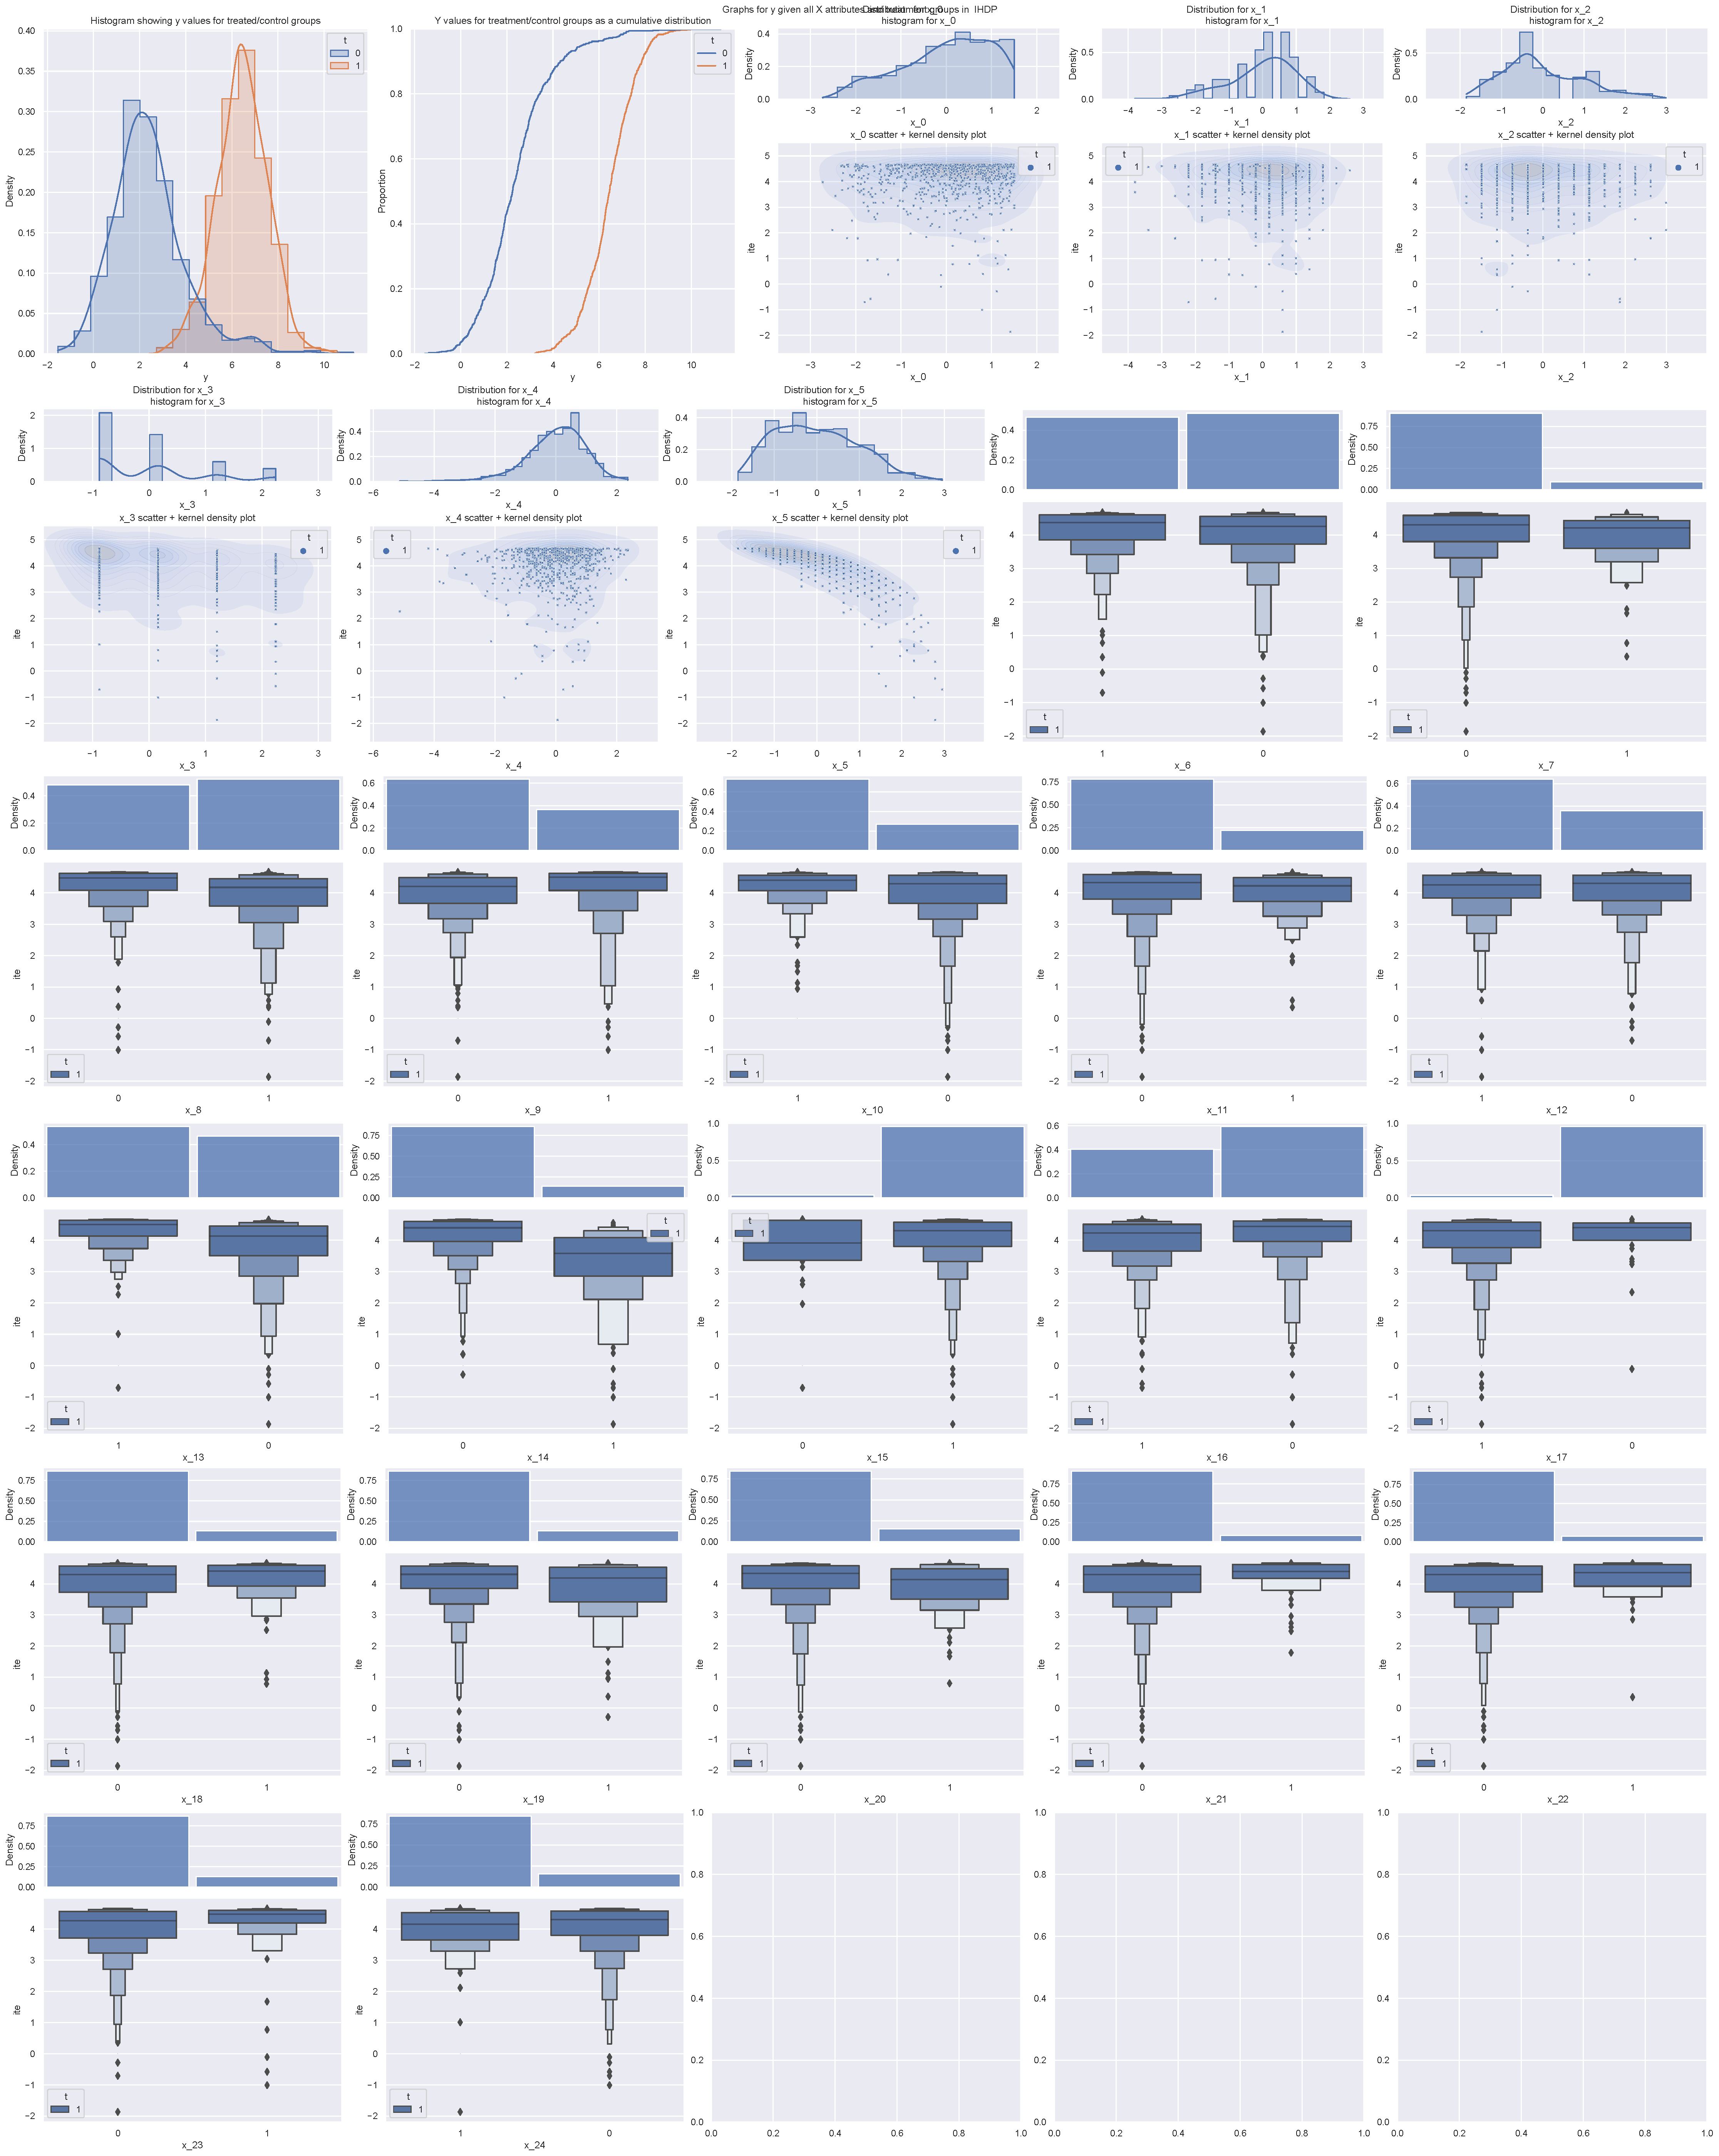
\includegraphics[width=1\textwidth]{project/data/ihdp_graphs.pdf}
    \caption{
        \label{fig:ihdpgraphs}Several graphs for the IHDP dataset, including counterfactuals
    }
\end{figure}

These graphs show how the \texttt{ite} values (along with \texttt{t0} and \texttt{t1})
vary for each individual, based on the value of each \texttt{x} variable for each individual. \texttt{t0}, \texttt{t1}, and \texttt{ite} are based on known counterfactual
data (end result being that \texttt{t0} contains the \texttt{y} value for the case where
the individual was in the control group, and vice versa for \texttt{t1}).

Looking at the density/regression plot between \texttt{t0} and \texttt{t1}, 
we can see a general improvement in the \texttt{y} scores for the population when
receiving the treatment, with few individuals falling below the \texttt{y=x diagonal}
line (these individuals being those who had a negative \texttt{ite}).

We can see a somewhat clear negative correlation between \texttt{x5} and \texttt{ite},
and we can also see that, for several of the binary-valued \texttt{x} values,
there is a rather large imbalance in the quantities of individuals in the dataset
who have each value, which could limit the amount of useful information we could
potentially gain from these variables.

\FloatBarrier

\begin{figure}[H]
    \centering
    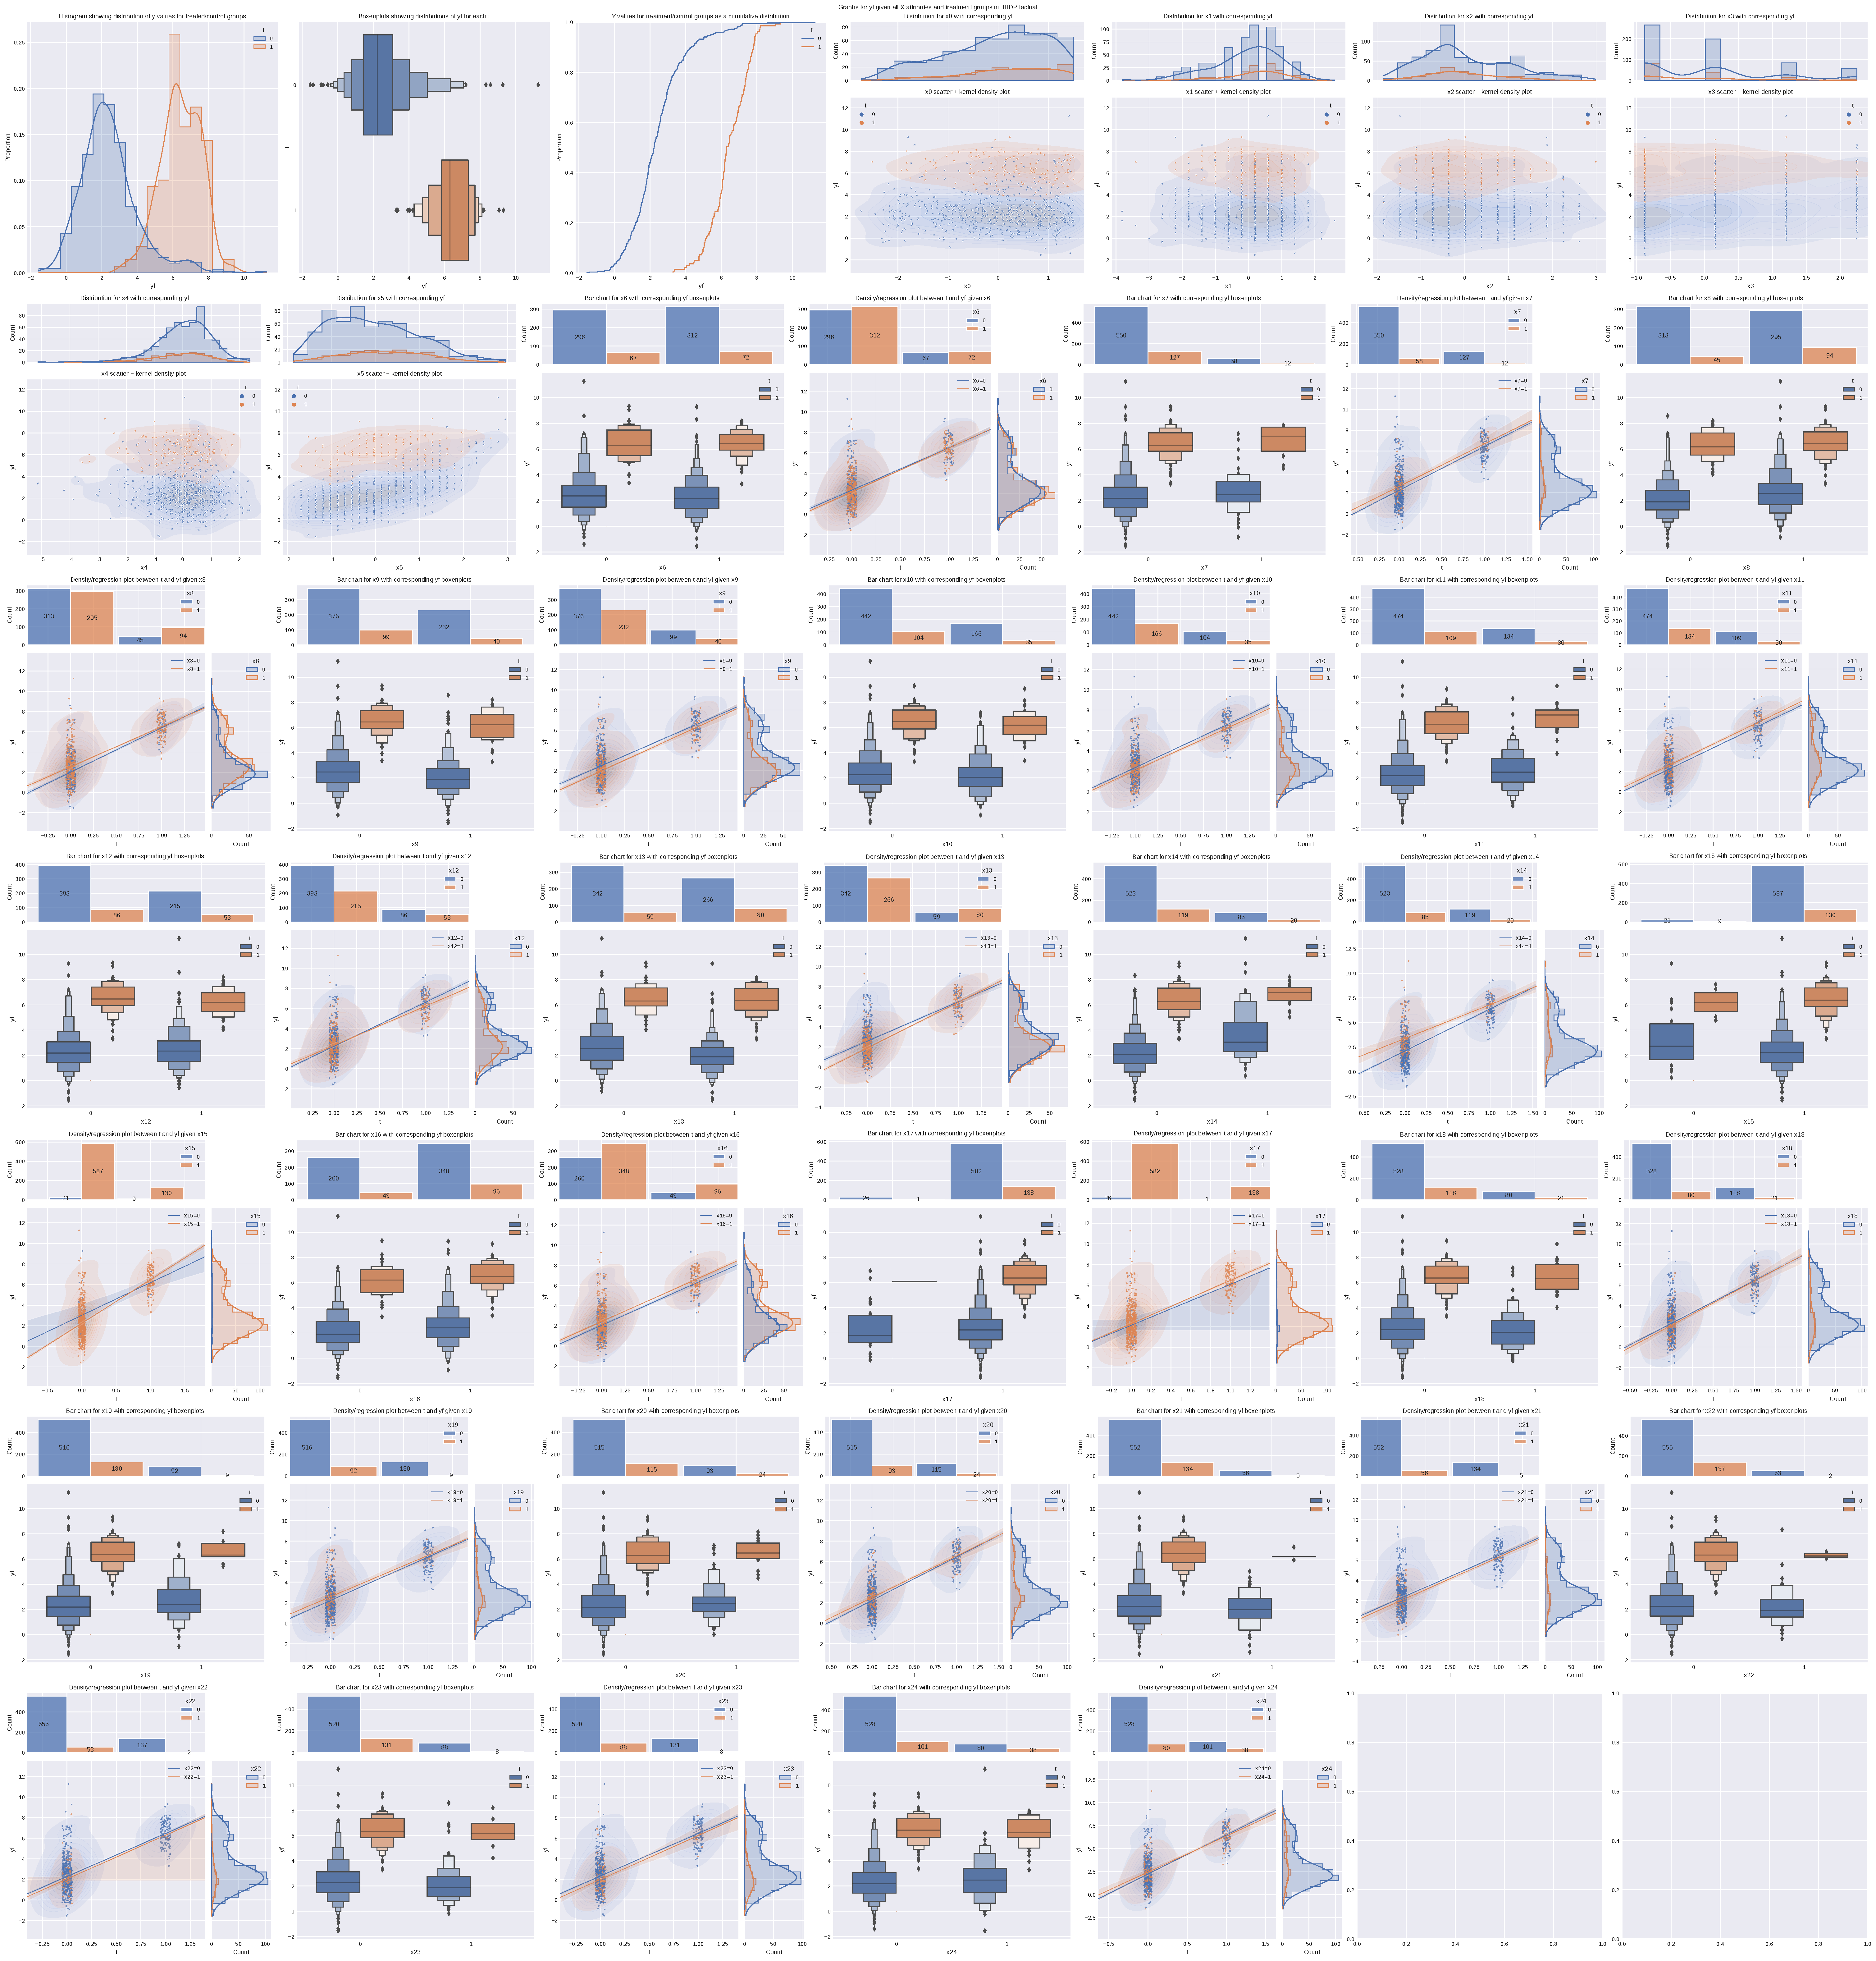
\includegraphics[width=1\textwidth]{project/data/ihdp_factuals.pdf}
    \caption{
        \label{fig:ihdpfact}Graphs for the factual data in IHDP
    }

\end{figure}

These graphs are of the factual data (\texttt{yf}) within the IHDP dataset.
These do illustrate the general positive correlation between individuals receiving
treatment and having a higher \texttt{yf} value, but also shows how imbalanced
this dataset is (most notably with \texttt{x17}, where only 27 individuals have
\texttt{x17==0}.
        
These graphs clearly illustrate that the treated individuals generally have higher
\texttt{yf} values than their untreated peers, with roughly similar interquartile
ranges for treatment/control groups with different values for each binary
\texttt{x} value (even in the extremely unbalanced cases).

\FloatBarrier

\begin{figure}[H]
    \centering
    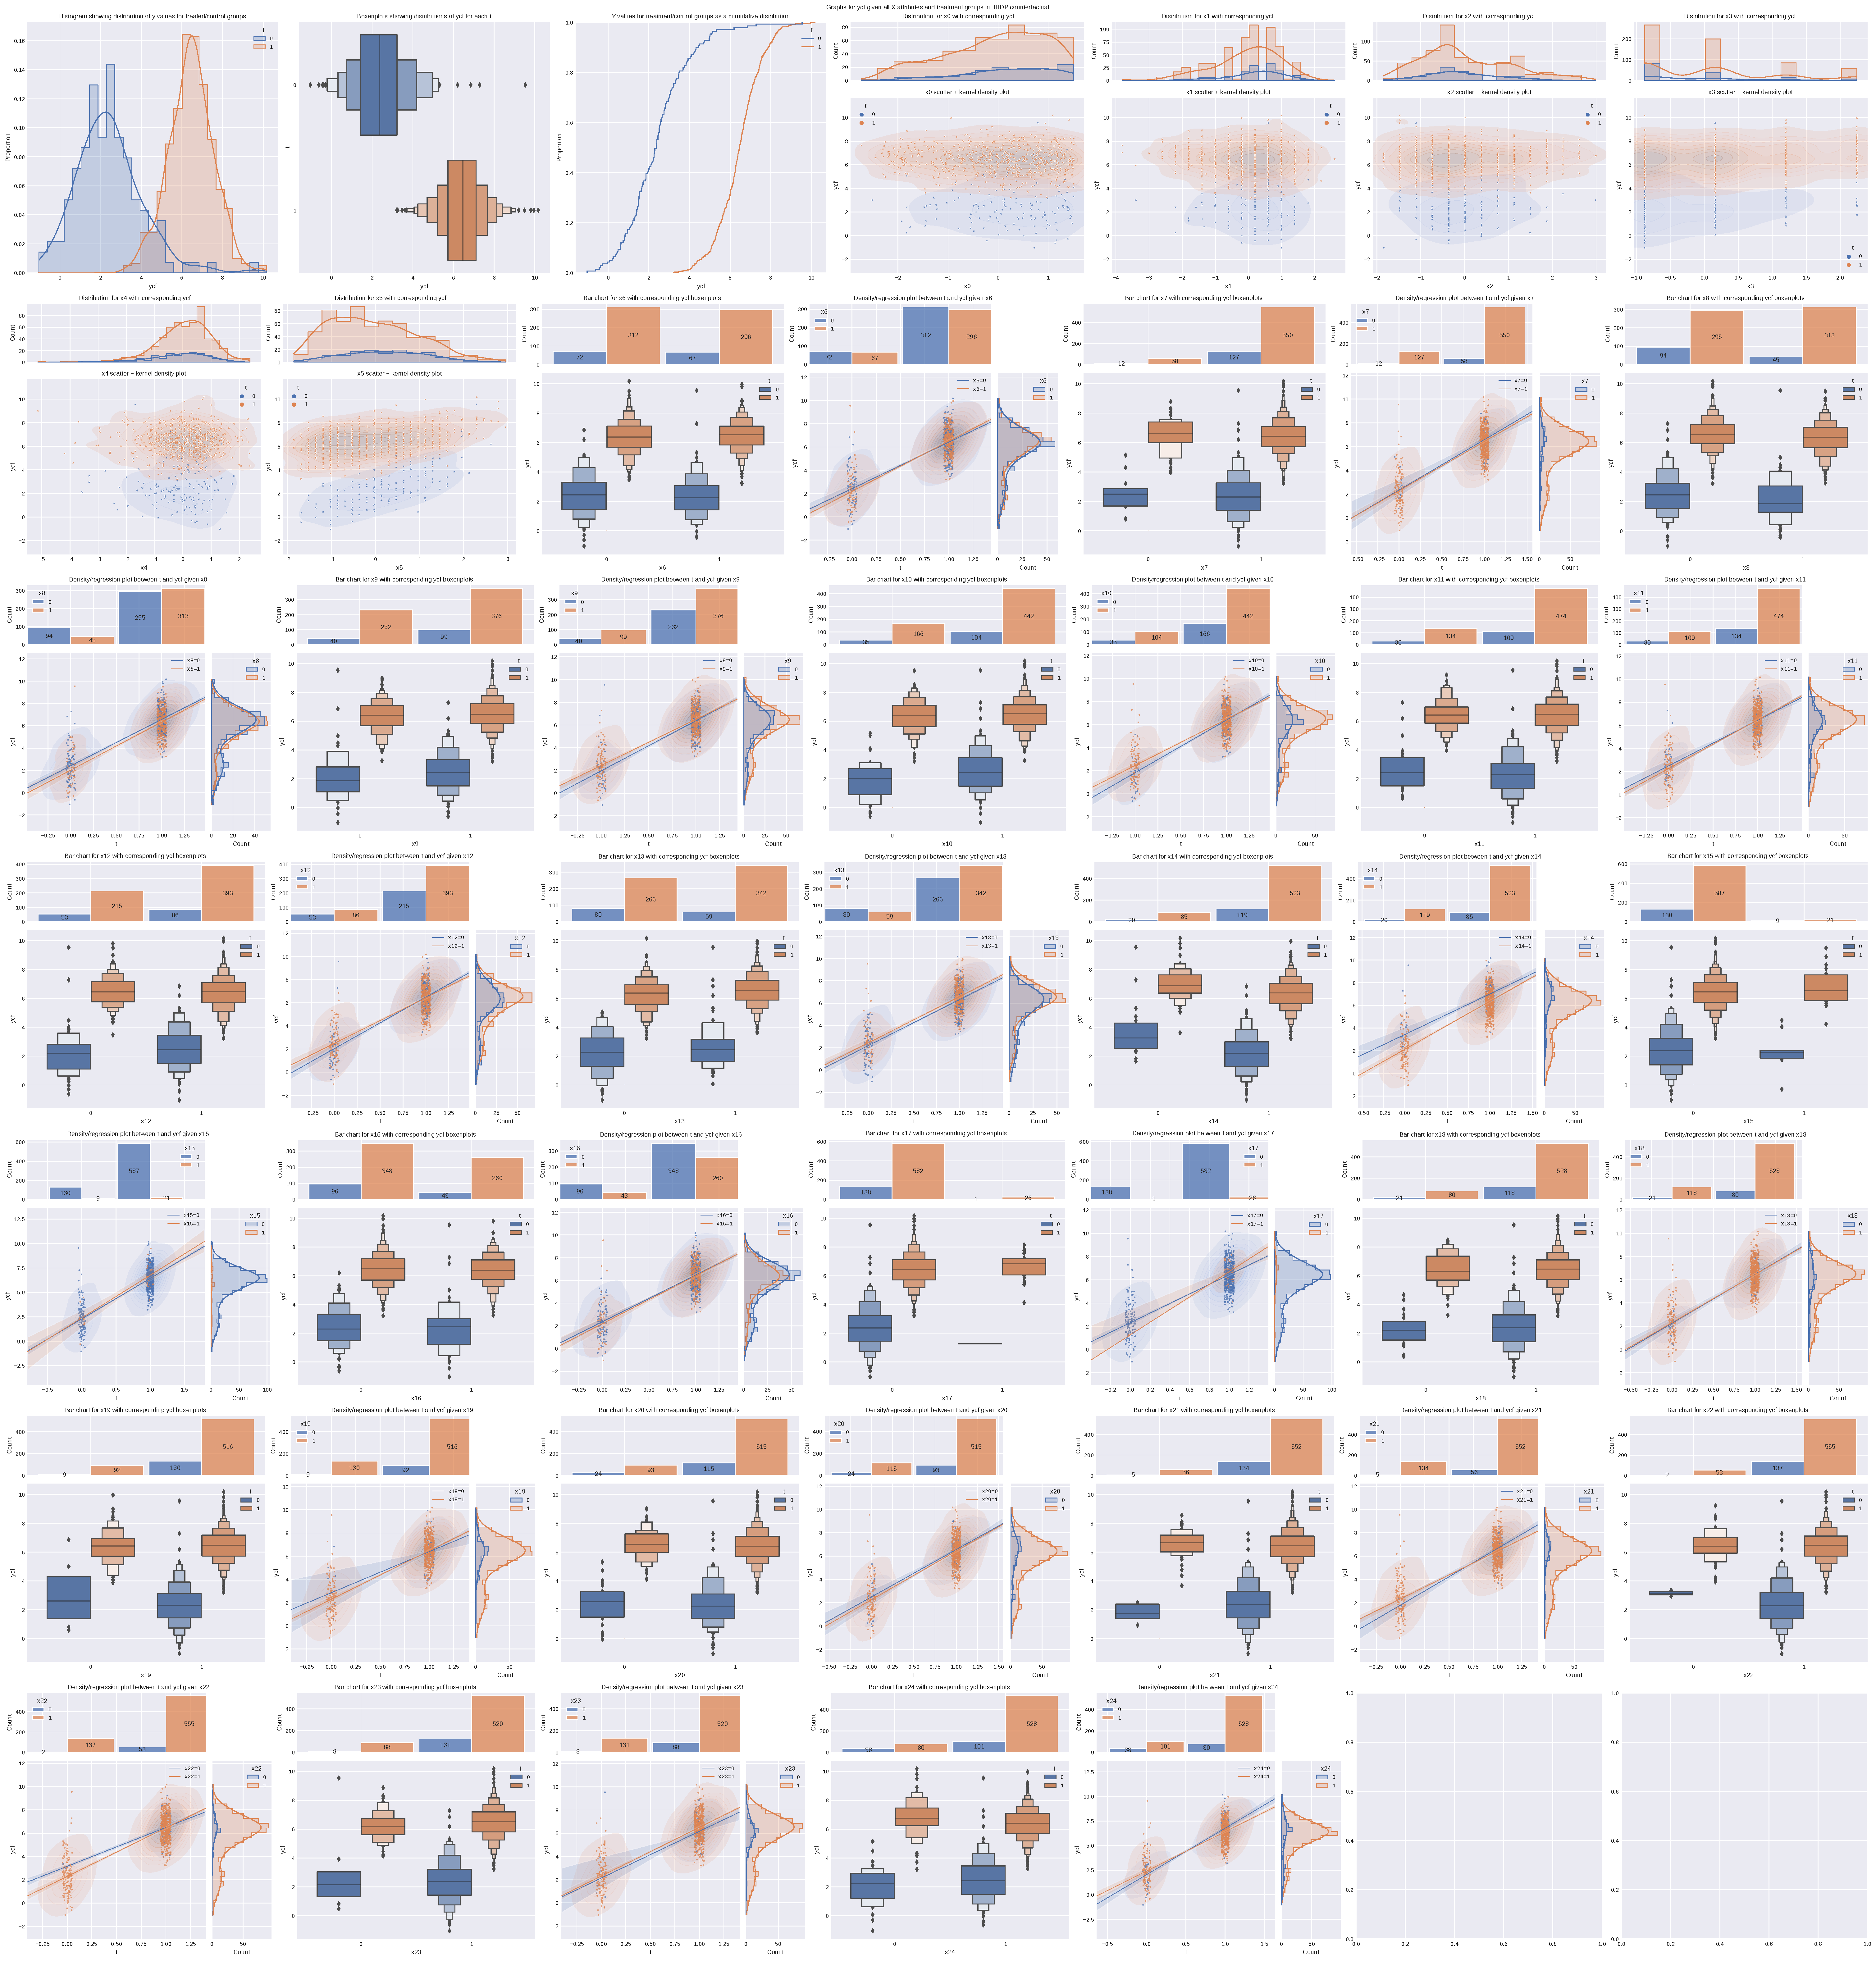
\includegraphics[width=1\textwidth]{project/data/ihdp_counterfactuals.pdf}
    \caption{\label{fig:ihdpcf}Graphs for the counterfactual data in IHDP}
\end{figure}

\FloatBarrier

\subsection{JOBS dataset visualizations}


Here are the graphs for the JOBS dataset.

\FloatBarrier

\begin{figure}[H]
\centering
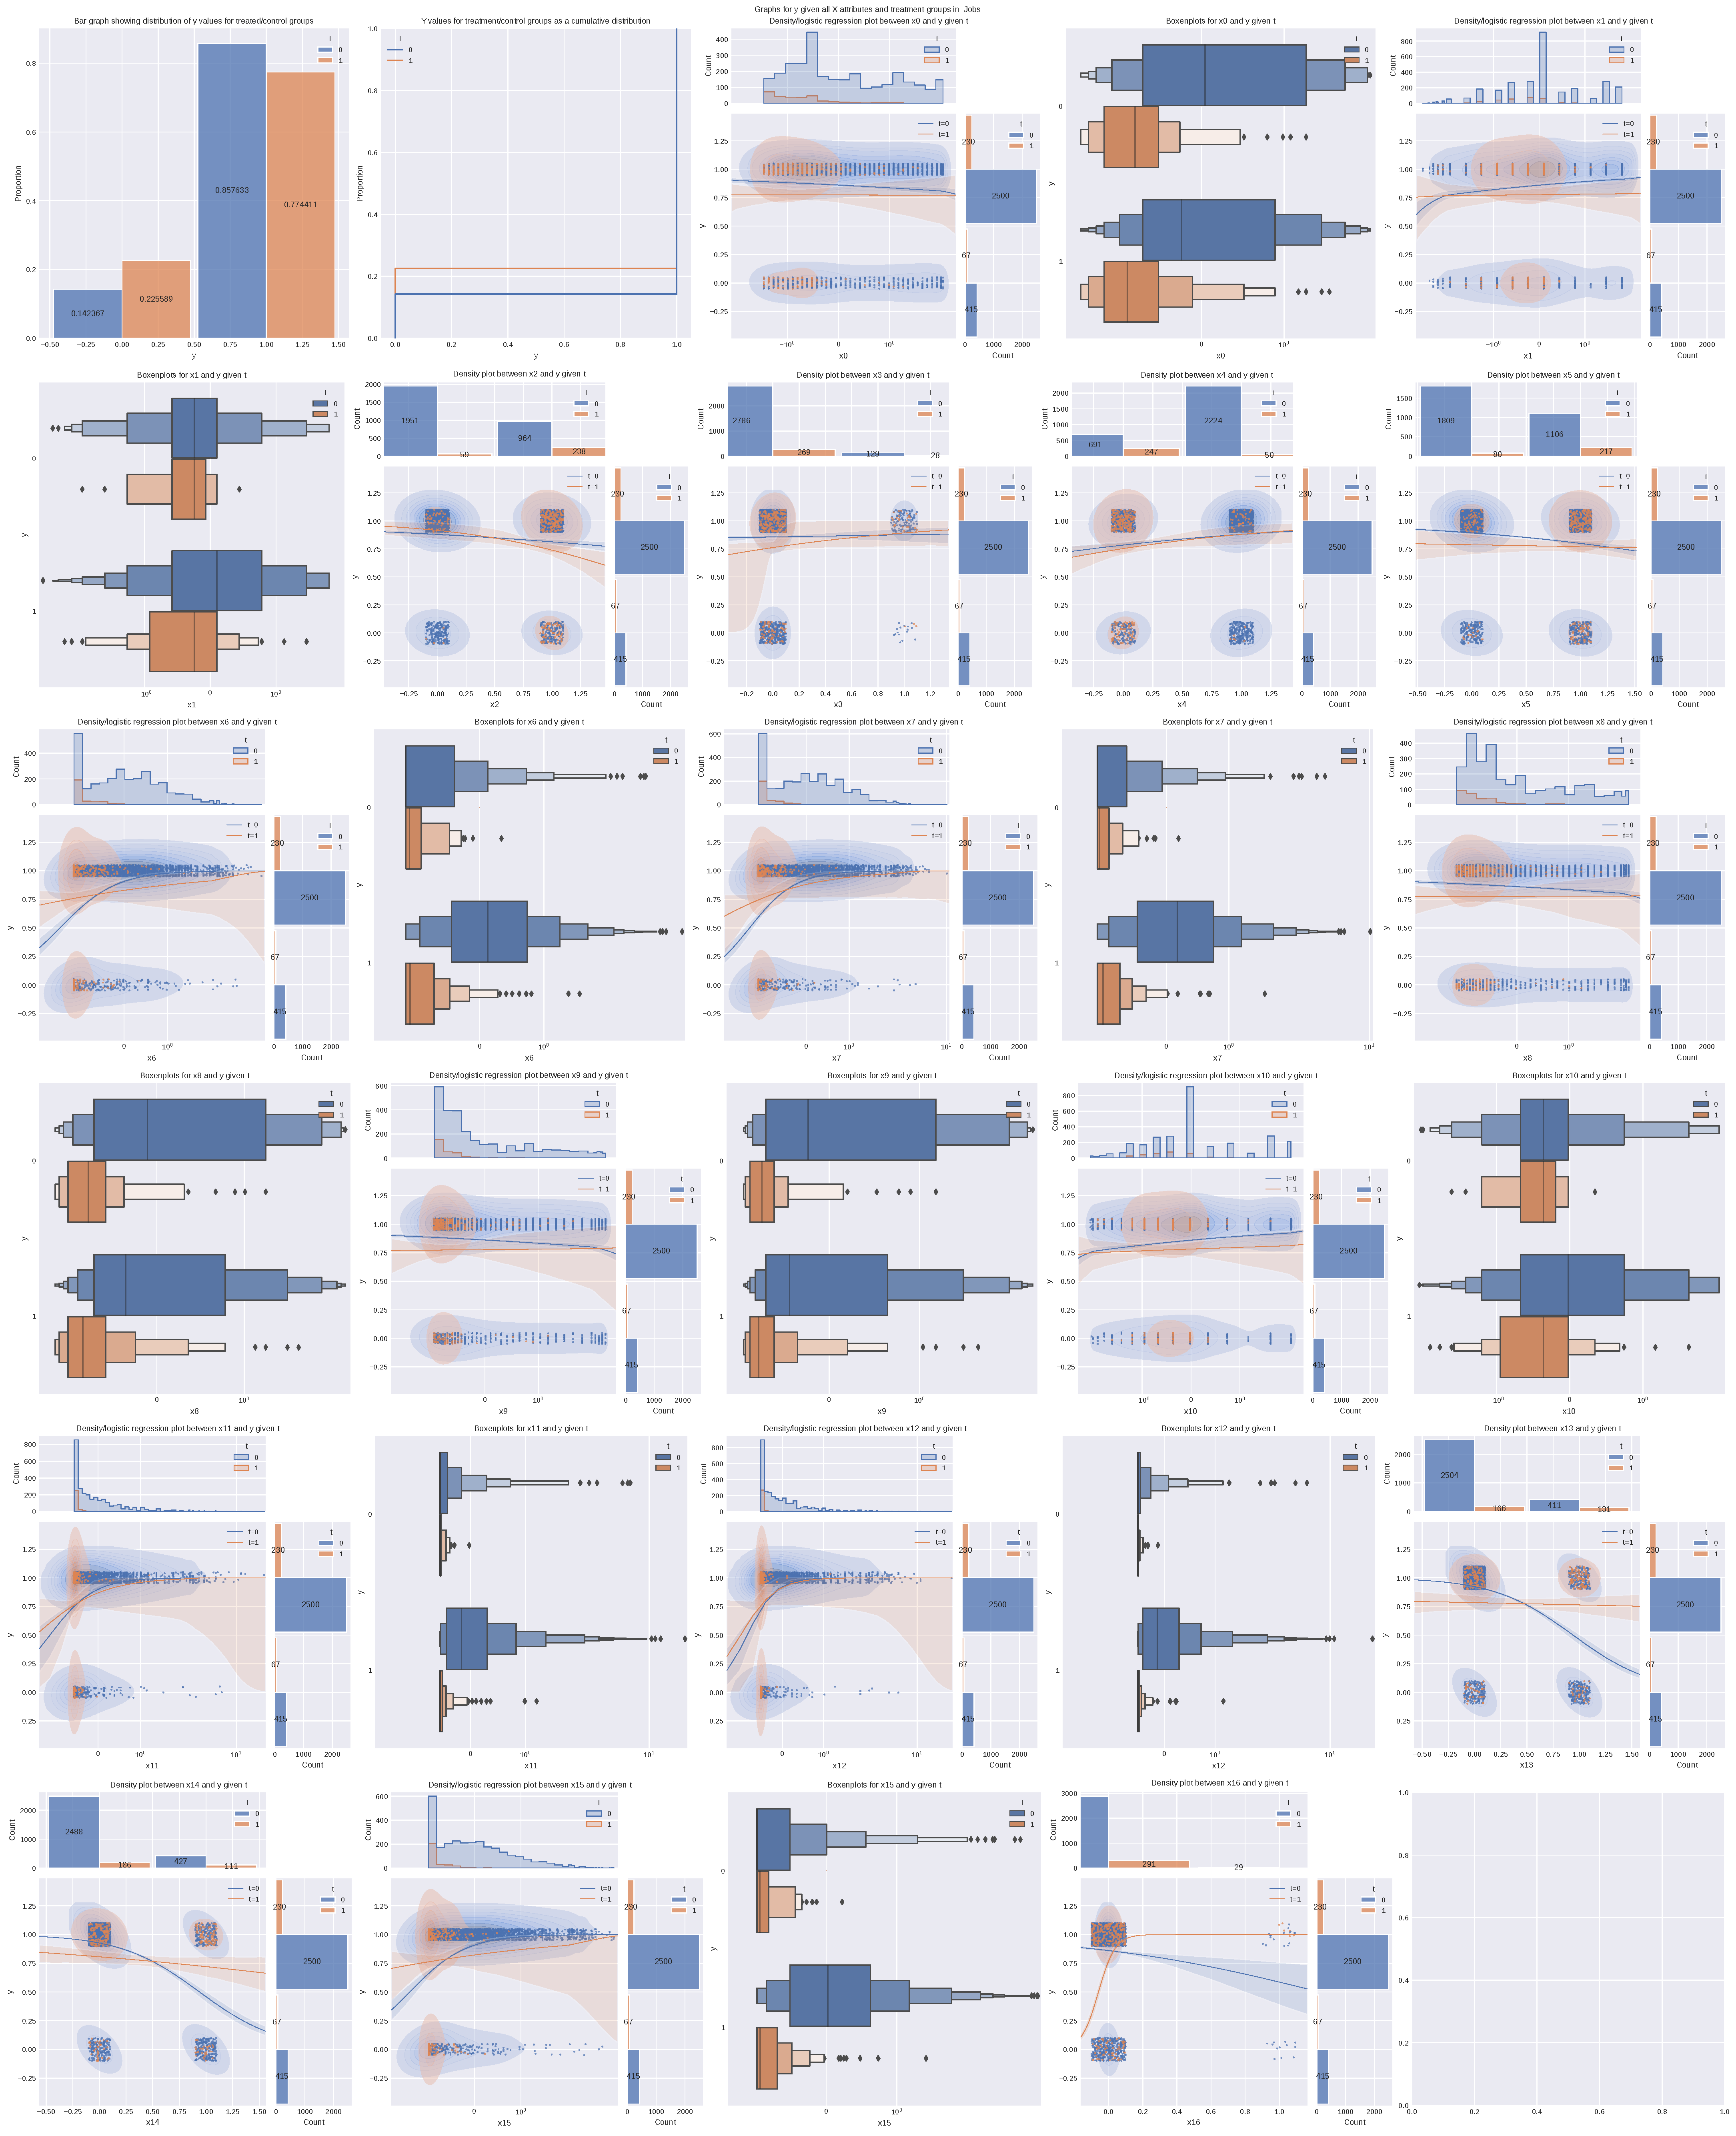
\includegraphics[width=1\textwidth]{project/data/jobs_graphs.pdf}
\caption{\label{fig:jobsgraphs}Several graphs for the JOBS dataset}
\end{figure}

\FloatBarrier

\quoteOFF
\printbibliography


\end{document}